\documentclass[12pt]{article}

% Ћирилица: кодирање фонта и језик (српски, ћирилица)
\usepackage[T2A]{fontenc}
\usepackage[utf8]{inputenc}
\usepackage[serbianc]{babel}

% Величина стране и маргине
\usepackage[a4paper,top=2cm,bottom=2cm,left=2.5cm,right=2.5cm]{geometry}

% Корисни пакети
\usepackage{amsmath}
\usepackage{enumitem}
\usepackage{float}
\usepackage{booktabs}
\usepackage{tcolorbox}
\tcbuselibrary{breakable}
\usepackage[colorlinks=true, allcolors=blue]{hyperref}

% Цртање електричних кола (европски симболи)
\usepackage[european]{circuitikz}
\usetikzlibrary{babel}

% Оквир за решене примере
\newtcolorbox[auto counter]{primer}{breakable,
    colback=white, colframe=black!55, colbacktitle=black!55, coltitle=white,
    fonttitle=\bfseries\small, title={Пример~\thetcbcounter},
    boxrule=0.5pt, arc=1.5pt, left=6pt, right=6pt, top=3pt, bottom=3pt,
    before skip=8pt, after skip=10pt}

% Оквир за кључне формуле
\newtcolorbox{kljucno}{colback=blue!4, colframe=blue!45!black,
    boxrule=0.5pt, arc=1.5pt, left=8pt, right=8pt, top=4pt, bottom=4pt}

\title{Генерална функционалност система убризгавања ОТО мотора - пропитивање}
\author{Аутоелектронски системи 2}
\date{}

\begin{document}
\maketitle


\section{Коефицијент вишка ваздуха}

Бензин у мотор не довлачимо директно, већ прво довучено бензин под притиском претворимо у 
гасно агрегатно станје, односно у гас и онда  га мешамо са ваздухом. Таква комбинација горива
и ваздуха се зове \textbf{смеша}.

Потребно је најпре дефинисати \textbf{коефицијент вишка ваздуха} $\lambda$ (енг. Ламбда). 
Ламбда дефинишемо помоћу следеће формуле: 

\begin{equation}
    \lambda = \frac{\text{доведена количина ваздуха}}{\text{теоријски потребна количина ваздуха}}
\end{equation}

\textbf{Теоријски потребна величина ваздуха} је тзв. стехеометријски однос мешавине ваздуха и бензина.
Тај теоријски потребан однос је избоси приближно 1:14.7. Шта значи то? Како би мотор радио У
оптималном стању, на 1$kg$ је потребно довести 14.7$kg$ ваздуха. Како онда формула која је написана 
горе функционише? 

\begin{itemize}
    \item $\lambda = 1$, направљена је савршен однос смеше
    \item $\lambda < 1$, доведена количина ваздуха је манје од теоријски потребне, смеша је \textbf{богатија горивом}
    \item $\lambda > 1$, доведена количина ваздуха је више од теоријски потребне, смеша је \textbf{сиромашнија горивом}
    \item $\lambda > 1.3$, мотор не може да се упали
\end{itemize}

\section{Подела система убризгавања}

Основна подела система убризгавања је по \textbf{методи регулације} и она чини: 

\begin{itemize}
    \item Хидро-механичка регулација - чисто механичка регулација убризгавања (K - Jetronic).
    \item Механичко електронска регулација - надоградња на механичку регулацију, додата
            електрика ради прецизније регулације (KE - Jetronic).
    \item Електронска регулација - управљање регулацијом помоћу електронске управљачке 
            јединице. Прикупља информације преко сензора и на тај начин одлучује о 
            концентрацији смеше.
\end{itemize}

Сви ови системи регулације важе за убризгавање у више тачака, биће више речи о томе.

Системи убризгавања такође се деле по \textbf{временској} и \textbf{просторној} основи, односно када и 
где убризгавају гориво.

Временска подела: 

\begin{itemize}
    \item Континуално убризгавање - Убризгава се гориво констрантно, под дејство притиска
    \item Симултано убризгавање - Гориво се убризгава понекад, али све бризгаљке одједном. Ради се помоћу електромагнетских бризгаљки.
    \item Групно убризгавање - Гориво се убризгава понекад, али само групе бризгаљки у исто време. Ради се помоћу електромагнетских бризгаљки.
    \item Секвенцијално убризгавање - Гориво се убризгава понекад, али свака бризгаљка појединачно. Ради се помоћу електромагнетских бризгаљки.
\end{itemize}

Просторна подела: 

\begin{itemize}
    \item Убризгавање у више тачака (MPI) - место убризгавања је непосредно пре простора за сагоревање.
        На овај начин засебно за сваки простор за сагоревање добијамо потребну мешавину.
    \item Централно убризгавање (SPI) - убрзгавање се ради преко једне бризгаљке, на место довођења
        горива, тако да се у простор за сагоревање увелико уноси мешавина готива и
        ваздуха, без засебног мешања.
    \item Директно убризгавање место убризгавања је у простору за сагоревање. Бенефит оваквог
        начин убрзигавање је то што у простор за сагоревање уносимо само ваздух, а додајемо гориво накнадно.
        На тај начин, на зидовима мотора се не захвата слој горива и меша је прецизнија. Овакав
        начин мешања могући је само код потпуно електронских система мешања.
\end{itemize}

\begin{figure}[H]
    \centering
    \begin{minipage}{0.32\textwidth}
        \centering
        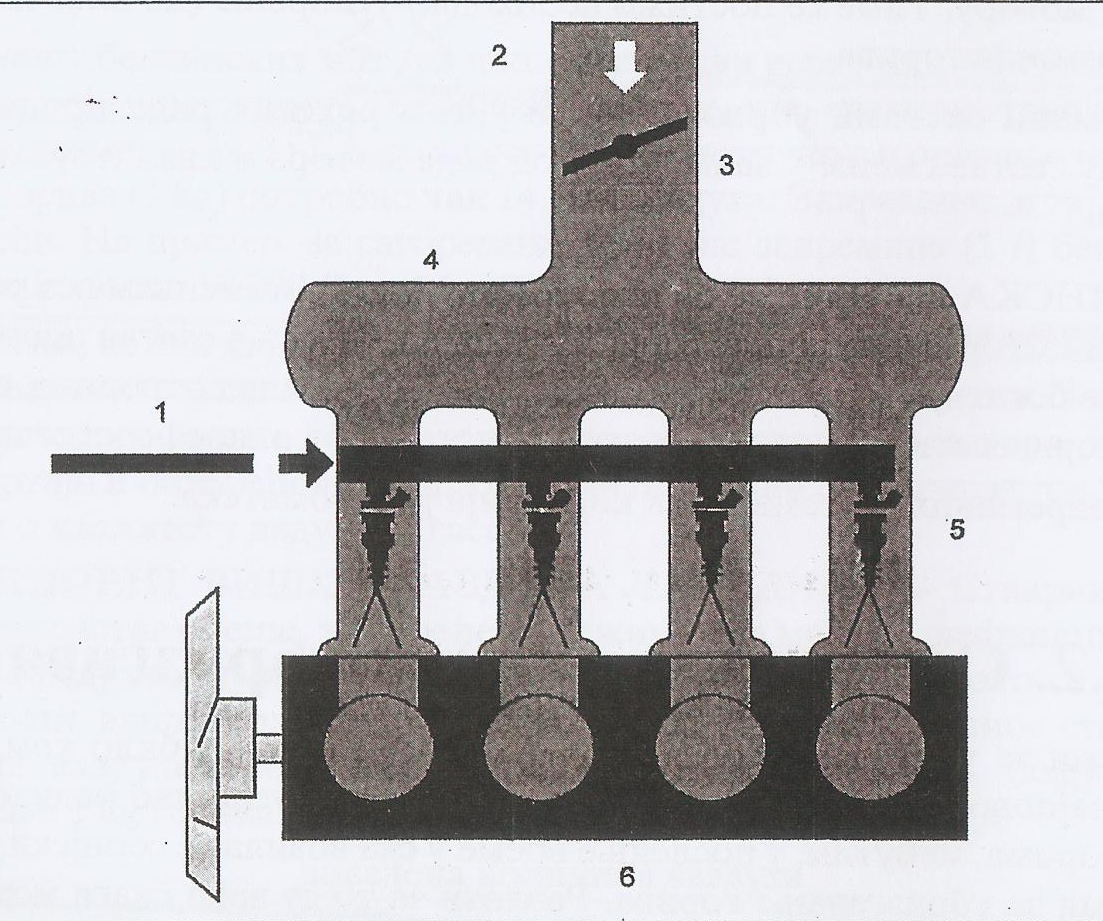
\includegraphics[width=\linewidth]{slike/engineE.png}
        \caption{Убризгавање у више тачака}
        \label{fig:slika1}
    \end{minipage}
    \hfill
    \begin{minipage}{0.32\textwidth}
        \centering
        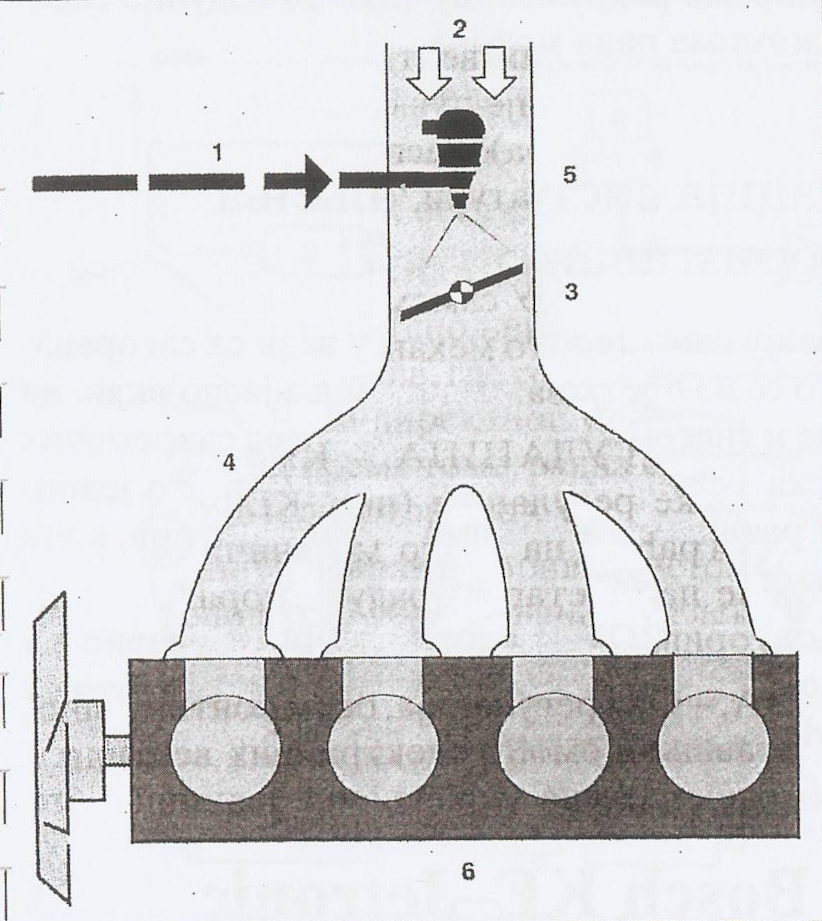
\includegraphics[width=\linewidth]{slike/engine2E.png}
        \caption{Централно убризгавање}
        \label{fig:slika2}
    \end{minipage}
    \hfill
    \begin{minipage}{0.32\textwidth}
        \centering
        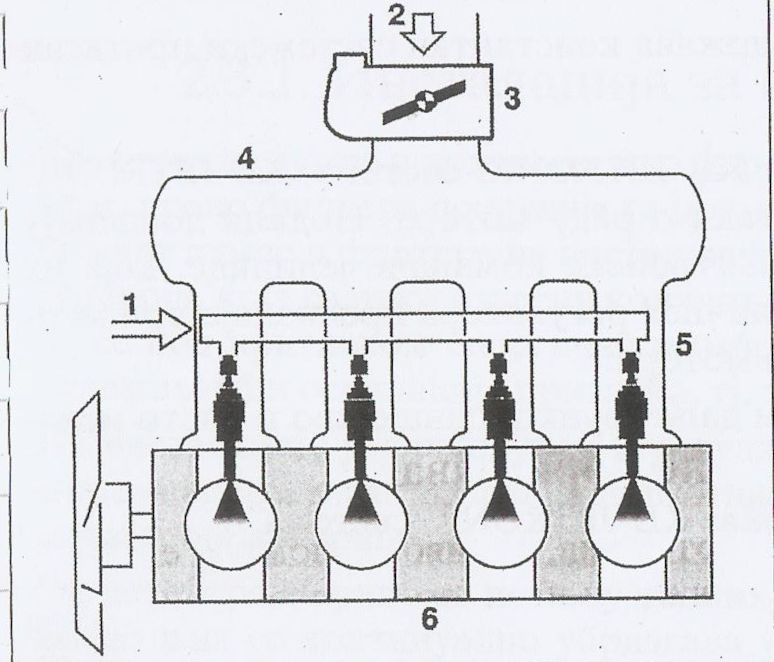
\includegraphics[width=\linewidth]{slike/engine2E2.png}
        \caption{Фиректно убризгавање}
        \label{fig:slika3}
    \end{minipage}
\end{figure}

\section{Контрола рада мотора прилагођавањем смеше}

\begin{table}[H]
\centering
\renewcommand{\arraystretch}{1.3}
\begin{tabular}{|l|c|}
    \hline
    \textbf{Режим рада} & $\boldsymbol{\lambda}$ \\ \hline
    \textbf{Хладан старт}         & $\lambda < 1$ \\ \hline
    \textbf{Загревање}            & $\lambda < 1$ \\ \hline
    \textbf{Празан ход}           & $\lambda < 1$ \\ \hline
    \textbf{Делимично оптерећење} & $\lambda \geq 1$ \\ \hline
    \textbf{Пуно оптерећење}      & $\lambda < 1$ \\ \hline
    \textbf{Убрзање}              & $\lambda < 1$ \\ \hline
    \textbf{Кочење мотором}       & $\lambda > 1$ \\ \hline
    \textbf{Висинска корекција}   & $\lambda \approx 1$ \\ \hline
\end{tabular}
\caption{Режими рада мотора и потребна вредност $\lambda$}
\label{tab:rezimi_lambda}
\end{table}

\end{document}